\documentclass{standalone}
\usepackage{amsmath}
\usepackage[dvipsnames]{xcolor}
\usepackage{tikz} 
\usetikzlibrary{arrows, decorations.markings,decorations.pathreplacing,angles,quotes}
\usepackage{microtype}
\usepackage{fourier}

\definecolor{nblue}{RGB}{31, 119, 180}

\begin{document}

\begin{tikzpicture}
   		\node[anchor=south west,inner sep=0] (Bild) at (0,0) {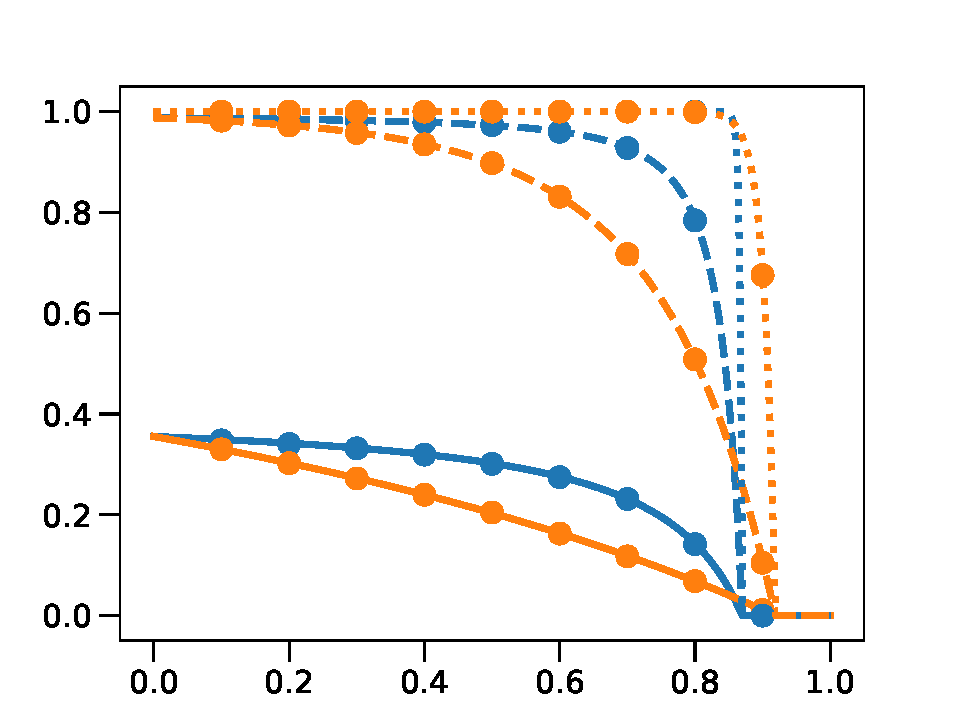
\includegraphics[scale=0.39]{fig2a_blank.pdf}};
   		\begin{scope}[x=(Bild.south east),y=(Bild.north west)]
			\node (right) at (1.5,0.5) {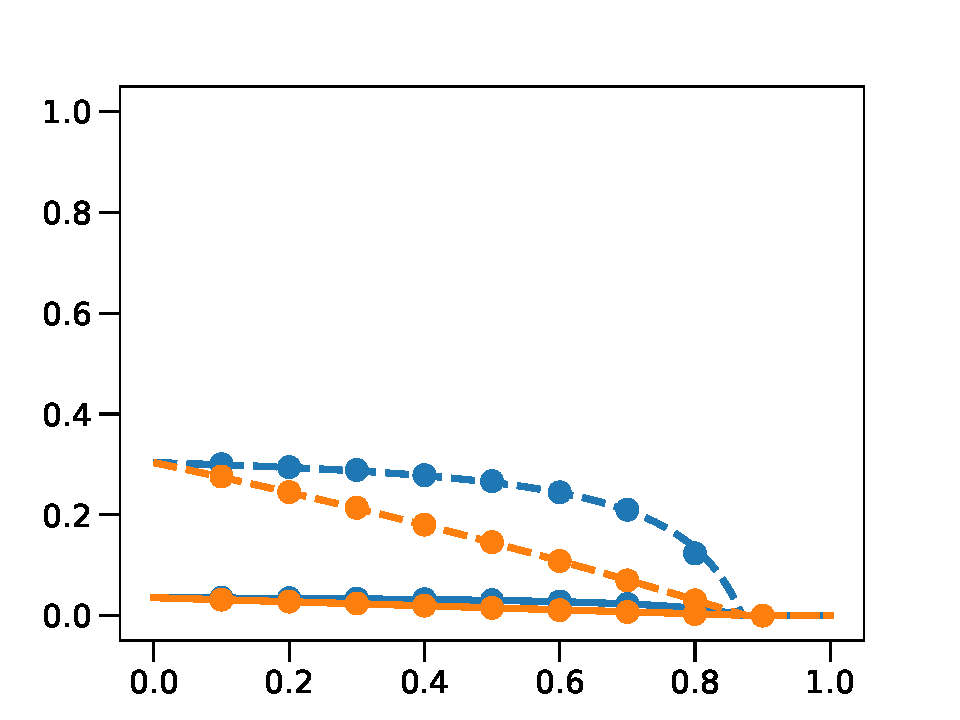
\includegraphics[scale=0.39]{fig2b_blank.pdf}}; 
			\node (right) at (0.5,-0.55) {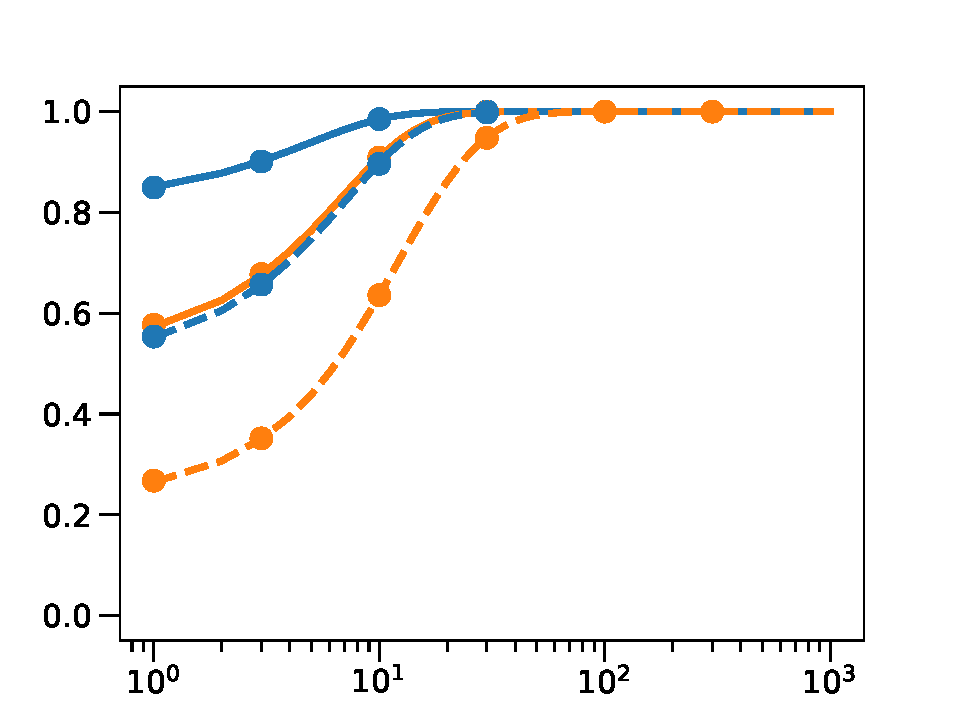
\includegraphics[scale=0.39]{fig2c_blank.pdf}};
			\node (right) at (1.5,-0.55) {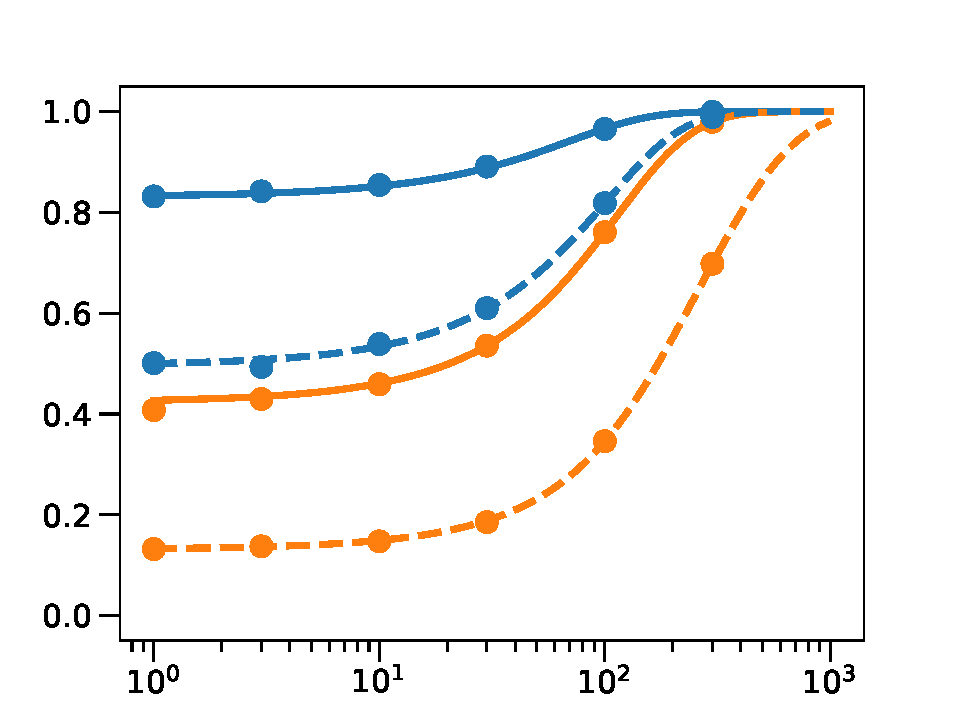
\includegraphics[scale=0.39]{fig2d_blank.pdf}};    
			  	
        	\draw (,-0.035) node {antiviral drug efficacy $\varepsilon_j$};
        	\draw (0.0,0.5) node [rotate=90] {est. probability $\varphi_j$};
        	\draw (0.0,-0.55) node [rotate=90] {rel. est. probability $\frac{\varphi_j}{\varphi}$};
        	\draw (,-1.1) node {inoculum size $V_0$};   
        	
        	\draw (0.52,0.95) node {LowN parameter set};
        	\draw (1.51,0.95) node {HighN parameter set};     	
        	
        	\draw[black,thick] (1.95,0.6) -- node[right=6pt] {\color{black} $V_0=1$} (2,0.6);
        	\draw[black,thick,dashed] (1.95,0.5) -- node[right=6pt] {\color{black} $V_0 = 10$} (2,0.5);
        	%\draw[black,thick,dotted] (1.95,0.4) -- node[right=6pt] {\color{black} $V_0 = 100$} (2,0.4);
        	
        	\draw[black] (0.85,0.82) node {\Large A};
        	\draw[black] (1.85,0.82) node {\Large B};
        	\draw[black] (0.85,-0.88) node {\Large C};
        	\draw[black] (1.85,-0.88) node {\Large D};
        	
        	%\draw[black,thick] (1.95,-0.4) -- node[right=6pt] {\color{black} $\varepsilon_j = 0$} (2,-0.4);
        	\draw[black,thick] (1.95,-0.55) -- node[right=6pt] {\color{black} $\varepsilon_j = 0.5$} (2,-0.55);
        	%\draw[black,thick] (1.95,-0.45) -- node[right=6pt] {\color{black} $\varepsilon_j = 0.25$} (2,-0.45);
        	\draw[black,thick,dashed] (1.95,-0.65) -- node[right=6pt] {\color{black} $\varepsilon_j = 0.75$} (2,-0.65);
        	
        	\draw[nblue,thick] (0.2,-1.2) -- node[right=10pt] {\color{black} reducing viral production $p$} (0.3,-1.2);
        	\draw[orange,thick] (1.2,-1.2) -- node[right=10pt] {\color{black} reducing infectivity $\beta$} (1.3,-1.2);
    		\end{scope}
\end{tikzpicture}

\end{document}